% TODO: Remove
\addbibresource{../report.bib}

\chapter{Evaluation and Testing}

In the following section, we outline how we will be evaluating the suggested model.
Next, we will perform that evaluation and present the final results.

\section{Experimental Setup}

Since our deep model requires a large amount of computation, we like to make use of parallelization.
Hence, all of our experiments that involve the sequence-to-sequence model have been run on an \textit{Amazon EC2 p2.xlarge} instance.
This VM has a \textit{NVIDIA K80 GPU} with 12 GiB of GPU memory.
This instance was then setup with \textit{CUDA 8} and \textit{cuDNN v5.1} \cite{tensorflow,nvidia_developer_2017}.

The rest of the experiments are run on a 2016 MacBook Pro, with a 2.9GHz Intel Core i5 and 8GB of RAM, running MacOS 10.12.
To make sure that the same Python environment is used on both these machines, we consistently use \textit{Python 3.6} and a \textit{virtual environment} for the python dependencies.

As previously mentioned, the main dataset that will be used is \texttt{GRESCHBACH} but we will also be using some of the data in the \texttt{WANG14} dataset to see how the model performs on data that was recorded under different circumstances.
From both these datasets, we will only be using the preprocessed Tor cells and not the raw TCP traffic data.

% TODO: Should I include more here?

\section{Evaluation Techniques}

There are several different manners in how we can evaluate the feature selection process.
First of all, we could analyse the training and test error, as the model learns.
If the training curve suddenly drops, the learning rate might be too high.
Or if the space between both the training and the test error increases, the model will clearly be overfitting.

However, these graphs only show us how well the model is at reproducing the trace from a fingerprint but now how well it performs in a WF attack.
For this we need to train a classifier and see how well it performs by using the metrics described in section \ref{sec:classifier-training}.

To be able to compare these fingerprints with hand-picked ones, we could run the classifier with hand-picked features and with the automatically generated ones.
These hand-picked features are often chosen by experts and after a careful analysis of what the most appropriate features are.
Hence, if the classifier with our fingerprints were to get similar results or even outperform the classifiers with the hand-picked features, we know that the sequence-to-sequence model has been successful.
For these results to be accurate, we do not change any parameters within the classifiers.
Thus everything, except for the features, stays fixed.

For the classifiers, we pick a small set of five existing models.
We aim to pick models that have had an influence on the WF field whilst also having a variety of different classifiers.
This set includes the two \textit{support vector classifiers} (SVCs) used by Panchenko et al. \cite{panchenko1,panchenko2},
the k-fingerprinting attack, which relies on a \textit{random forest} (RF) used by Hayes et al. \cite{kfingerprinting}
and finally the \textit{k-nearest neighbours} (kNN) classifier used by Wang et al. \cite{wang_cai_johnson_nithyanand_goldberg_2014}.

For all of these models, we extract the exact same features as outlined in the respective papers and compare the performance of our generated features compared to the hand-picked ones.
The code for this feature extraction process can be found in the \texttt{feature\_extraction} module.
After analysing all of these features, the most important ones seem to be \cite{panchenko1,panchenko2,kfingerprinting,wang_cai_johnson_nithyanand_goldberg_2014}:

\begin{itemize}
  \item Total number of packets.
  \item Number of incoming packets.
  \item Number of outgoing packets.
  \item Percentage of incoming and outgoing packets.
  \item Concentration of packets.
\end{itemize}

We also aim to use the exact same hyperparameters described in the respective papers. More specifically:
\begin{itemize}
  \item \textbf{SVC} \cite{panchenko1} - a \textit{radial basis function} (RBF) kernel with $C = 2^{17}$ and $\gamma = 2^{-19}$.
  \item \textbf{SVC} \cite{panchenko2} - uses the same hyperparameters as in the previous SVC but with different features.
  \item \textbf{RF} \cite{kfingerprinting} - shows that the best accuracy/time tradeoff is made when $k = 3$ and $\textit{num\_trees} = 20$.
  \item \textbf{kNN} \cite{wang_cai_johnson_nithyanand_goldberg_2014} - also shows that the best accuracy/time tradoff is made when $k = 2$ and $k_{\textit{reco}} = 5$.
\end{itemize}

However, we do need to note that this might have an impact on the performance because these parameters have been specifically tuned for the hand-picked features and not for our fingerprints.

\section{Evaluation}

\subsection{Learning Parameter Tuning}

As mentioned in section \ref{sec:fingerprint-extraction-training}, there are a couple design decisions that need to be made regarding different architectures and learning parameters for the sequence-to-sequence model.
We first try to aim to get the appropriate values for the learning parameters within a simple encoder and decoder with LSTM cells and $120$ hidden states.

First, we start by varying the mini-batch sizes from $20$ to $400$ in steps of $20$.
The higher this value, the longer it takes before making a weight update and the lower the value, the more noise in the training data.
For instance, as can be seen in figure \ref{fig:varying-batch-sizes}, there is clearly a trend of the training error decreases over time.
However, since the batch size is low for the first case, there is a higher probability of having a batch where the training error is high for all of the samples within that batch.
Hence, the data will look very noisy.
Whilst the greater the batch size, the easier to spot this trend.
\begin{figure}[ht]
  \centering
  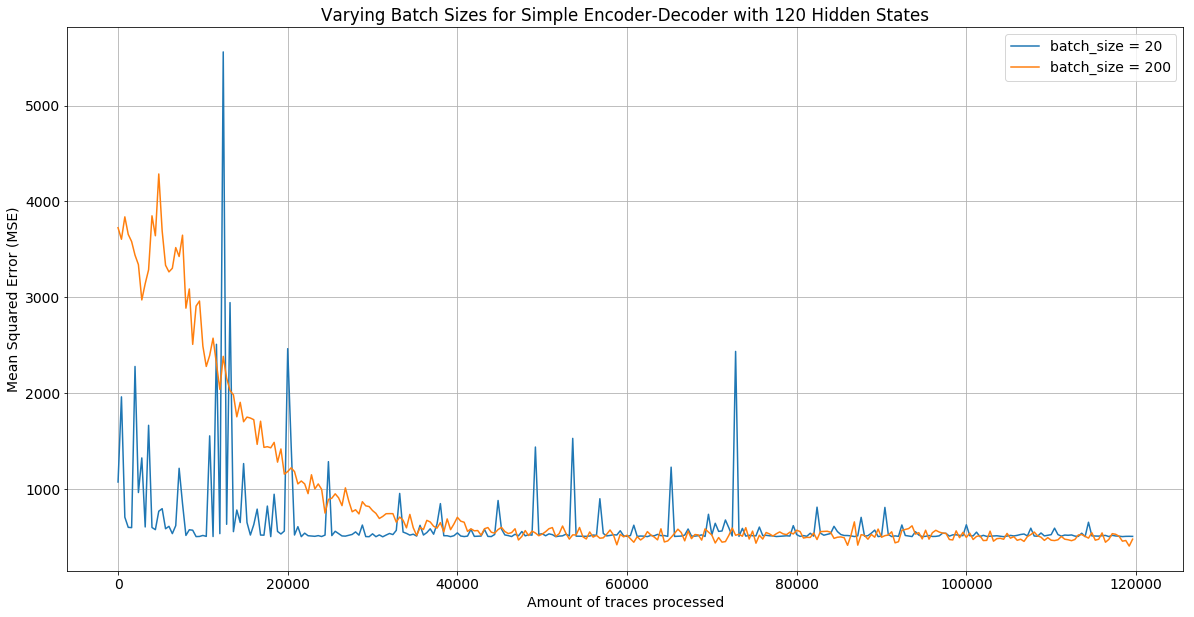
\includegraphics[width=0.9\textwidth]{varying-batch-sizes}
  \caption{Scaled MSE over traces processed for different batch sizes.}
  \label{fig:varying-batch-sizes}
\end{figure}

Preferably we would like to have an even greater batch size than $200$ but due to memory constraints, the model runs out of memory when the amount of hidden states is greater than $100$.
Thus through the rest of the report we will use a mini-batch size of $200$.

Next, we vary the learning rate $\gamma$ from $0.01$ to $0.000001$ with various optimizers (\textit{adam}, \textit{gradient descent} or \textit{RMSProp}) and loss functions (\textit{mean squared error (MSE)} or \textit{absolute loss} (AL)).
As expected, during our experiments, the \textit{adam optimizer} continuously demonstrated better results.

Next, we also noted that the best quality of data compression was achieved with a \textit{MSE loss functio}n and a learning rate of $0.000002$.
Hence, we set $\lambda = 0.000002$, $b = 200$ and use an adam optimizer with MSE for the rest of our experiments.

\subsection{Architecture Tuning}

Now that we have an average measure of the learning parameters, we can start changing the architecture of the sequence-to-sequence model to see which ones yield the best results.


% TODO: Include different 5 models as `subsubsection`

% Binary vs multiclass

\subsection{Classifier Performance}

% Include different models

% Did the design do the job you intended, or were there problems?
% Is your solution fit for purpose?
% How does the resulting system compare against the competition?


\section{Unit Tests}

On top of evaluating the results, we also needed to ensure that the results were in fact the the code behaves as we expect it to.
For this we use unit tests.
Some of the code, such as the sequence-to-sequence model is difficult to test but we can still test all of the preprocessing to see if that is correct.
For this we use Python's standard \texttt{unittest} module \cite{python_unittest_documentation}.
The reason for this choice is that it is flexible and the standard unit testing framework, which means it is commonly used.

On top of unit tests, \textit{Travis} was also used \cite{travis}.
Travis is a popular tool, that has an easy integration with Github, for continuous integration.
Therefore, every time a commit is pushed to the remote repository, Travis runs all of the tests automatically.
If one of the tests fails, Travis then automatically notifies all the contributors.

Finally, to check if our tests cover our entire codebase, \textit{codecov} is used \cite{codecov}.
This tool automatically checks how much of the codebase all of the unit tests cover.
At the time of writing, the coverage is $93\%$.
The bits that aren't covered by unit tests, such as the Tensorflow implementation of the sequence-to-sequence model, have been carefully examined to see if they behave as expected.
